%
% Cluster.tex
%
% History of LulzBot Printers
%
% Copyright (C) 2014, 2015 Aleph Objects, Inc.
%
% This document is licensed under the Creative Commons Attribution 4.0
% International Public License (CC BY-SA 4.0) by Aleph Objects, Inc.
%

\section{LulzBot 3D Printer Cluster}
This is the evolution of Aleph Object's LulzBot 3D Printer Cluster.

\begin{figure}[h!]
\thisfloatpagestyle{empty}
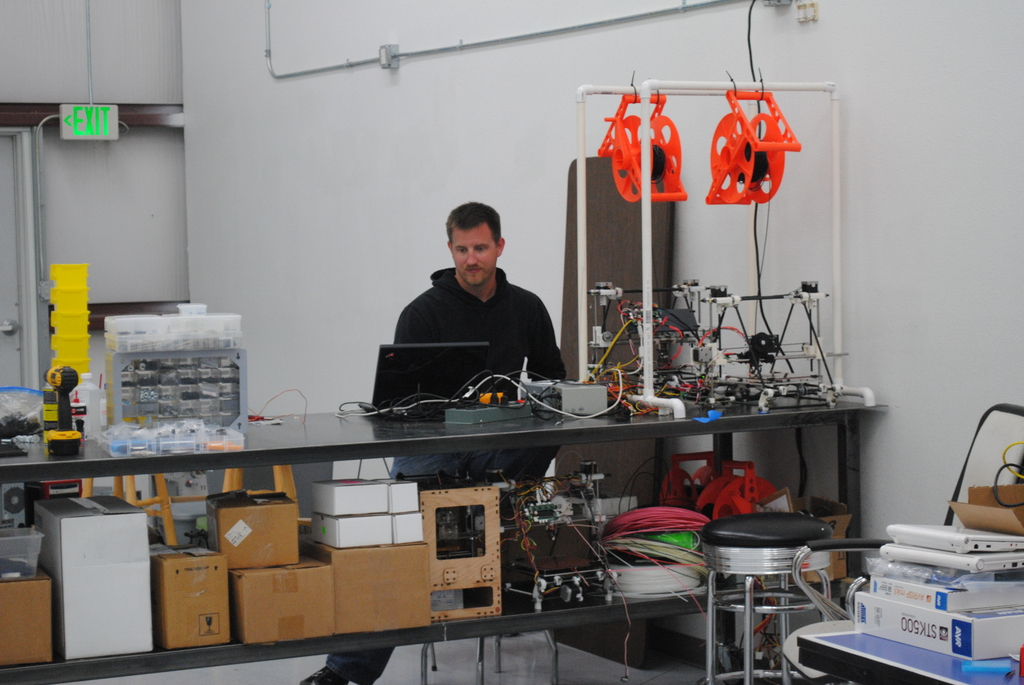
\includegraphics[keepaspectratio=true,height=0.40\textheight,width=1.00\textwidth,angle=0]{cluster/clonedel-2-node.jpg}
 \caption{3D Printer Cluster of 2 Mars Prusas, June, 2011.}
 \label{fig:clonedel-2-node}
\end{figure}

\begin{figure}[h!]
\thisfloatpagestyle{empty}
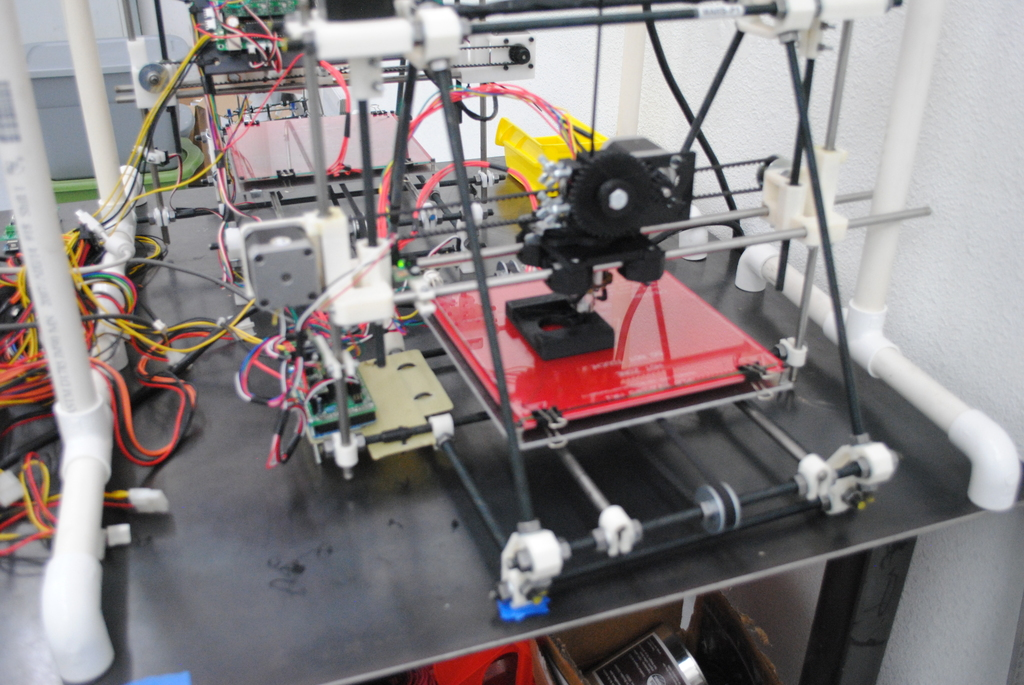
\includegraphics[keepaspectratio=true,height=0.40\textheight,width=1.00\textwidth,angle=0]{cluster/clonedel-2-node-close.jpg}
 \caption{3D Printer Cluster of 2 Mars Prusas Closeup.}
 \label{fig:clonedel-2-node-close}
\end{figure}

\begin{figure}[h!]
\thisfloatpagestyle{empty}
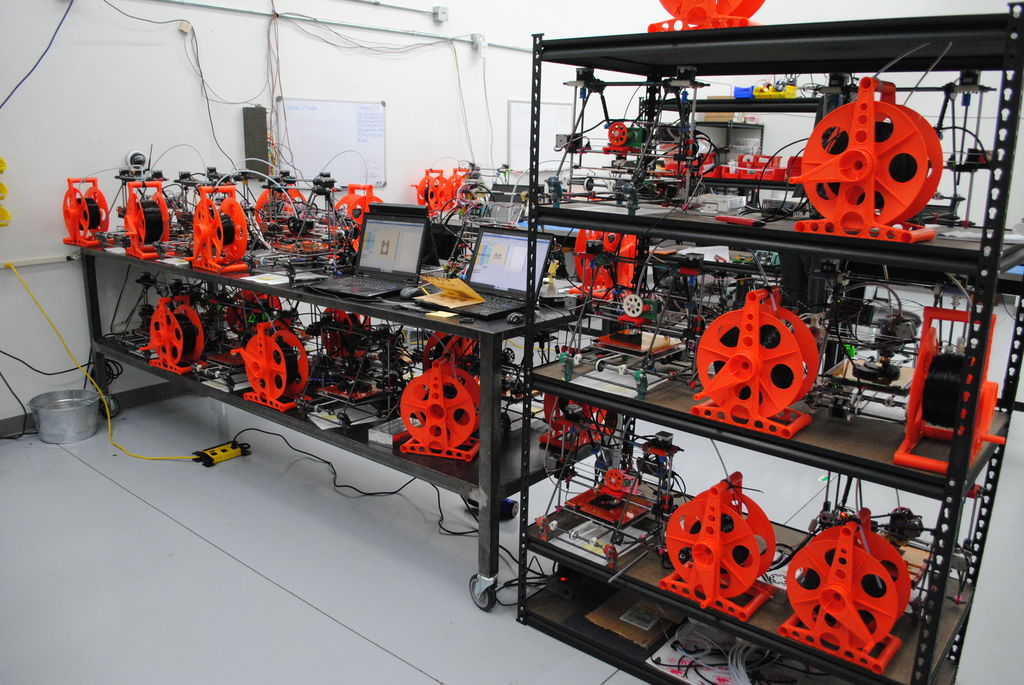
\includegraphics[keepaspectratio=true,height=0.40\textheight,width=1.00\textwidth,angle=0]{cluster/clonedel-19-node.jpg}
 \caption{3D Printer Cluster of 19 LulzBot Clonedels, October, 2011.}
 \label{fig:clonedel-20-node}
\end{figure}

\begin{figure}[h!]
\thisfloatpagestyle{empty}
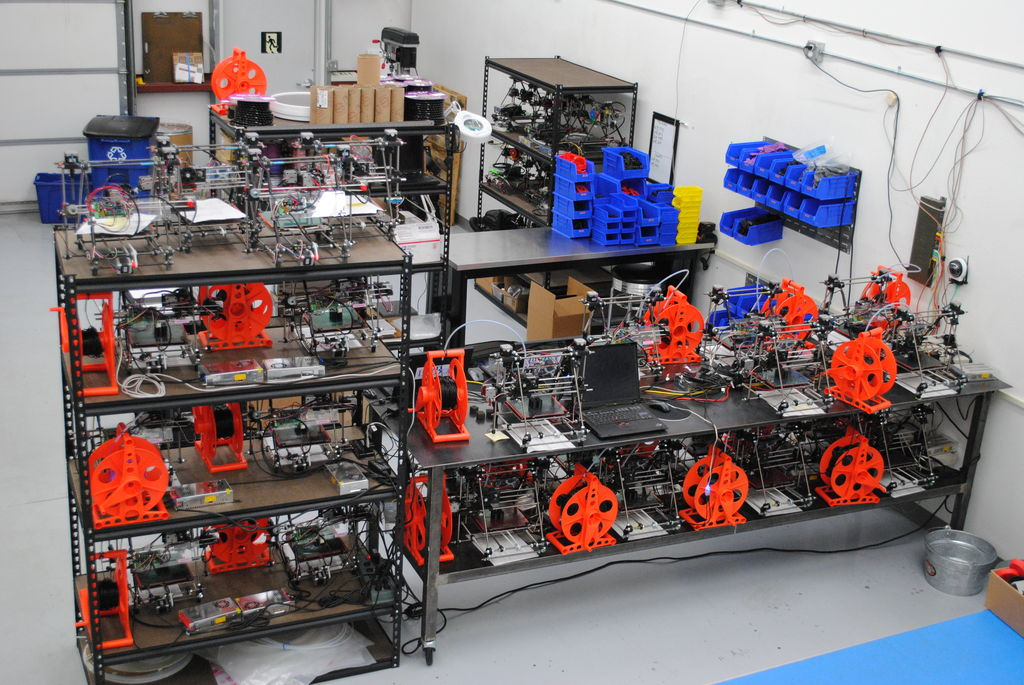
\includegraphics[keepaspectratio=true,height=0.40\textheight,width=1.00\textwidth,angle=0]{cluster/prusa-19-node-yearend.jpg}
 \caption{3D Printer Cluster of 19 LulzBot Prusas, December, 2011.}
 \label{fig:prusa-19-node-yearend}
\end{figure}

\begin{figure}[h!]
\thisfloatpagestyle{empty}
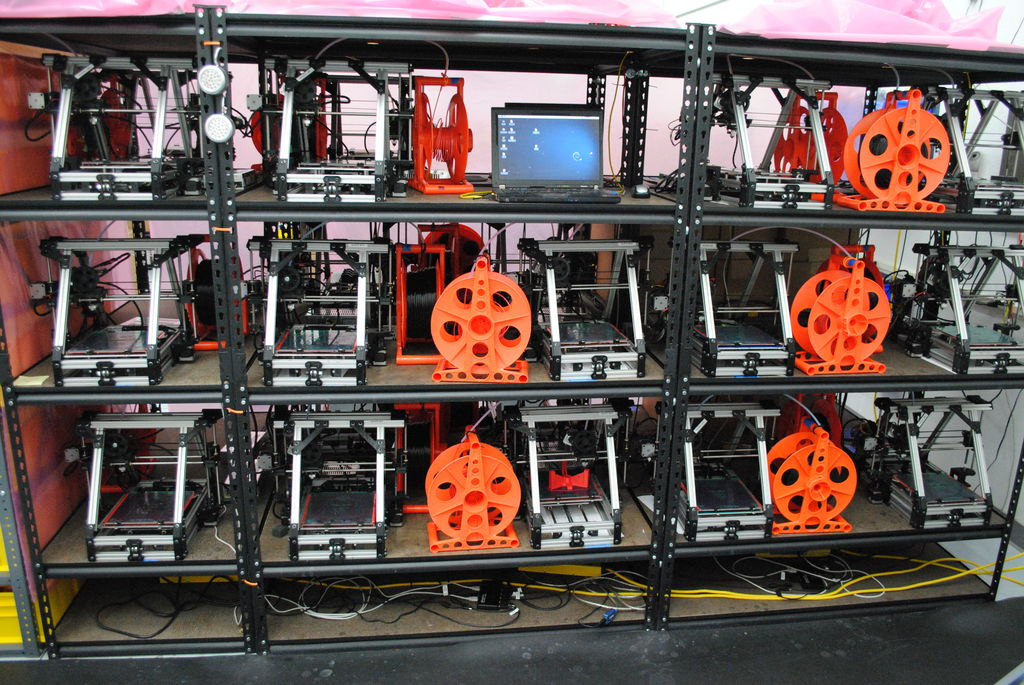
\includegraphics[keepaspectratio=true,height=0.40\textheight,width=1.00\textwidth,angle=0]{cluster/ao-28-node.jpg}
 \caption{3D Printer Cluster of 28 LulzBot AO-100s, July, 2012.}
 \label{fig:ao-28-node}
\end{figure}

\begin{figure}[h!]
\thisfloatpagestyle{empty}
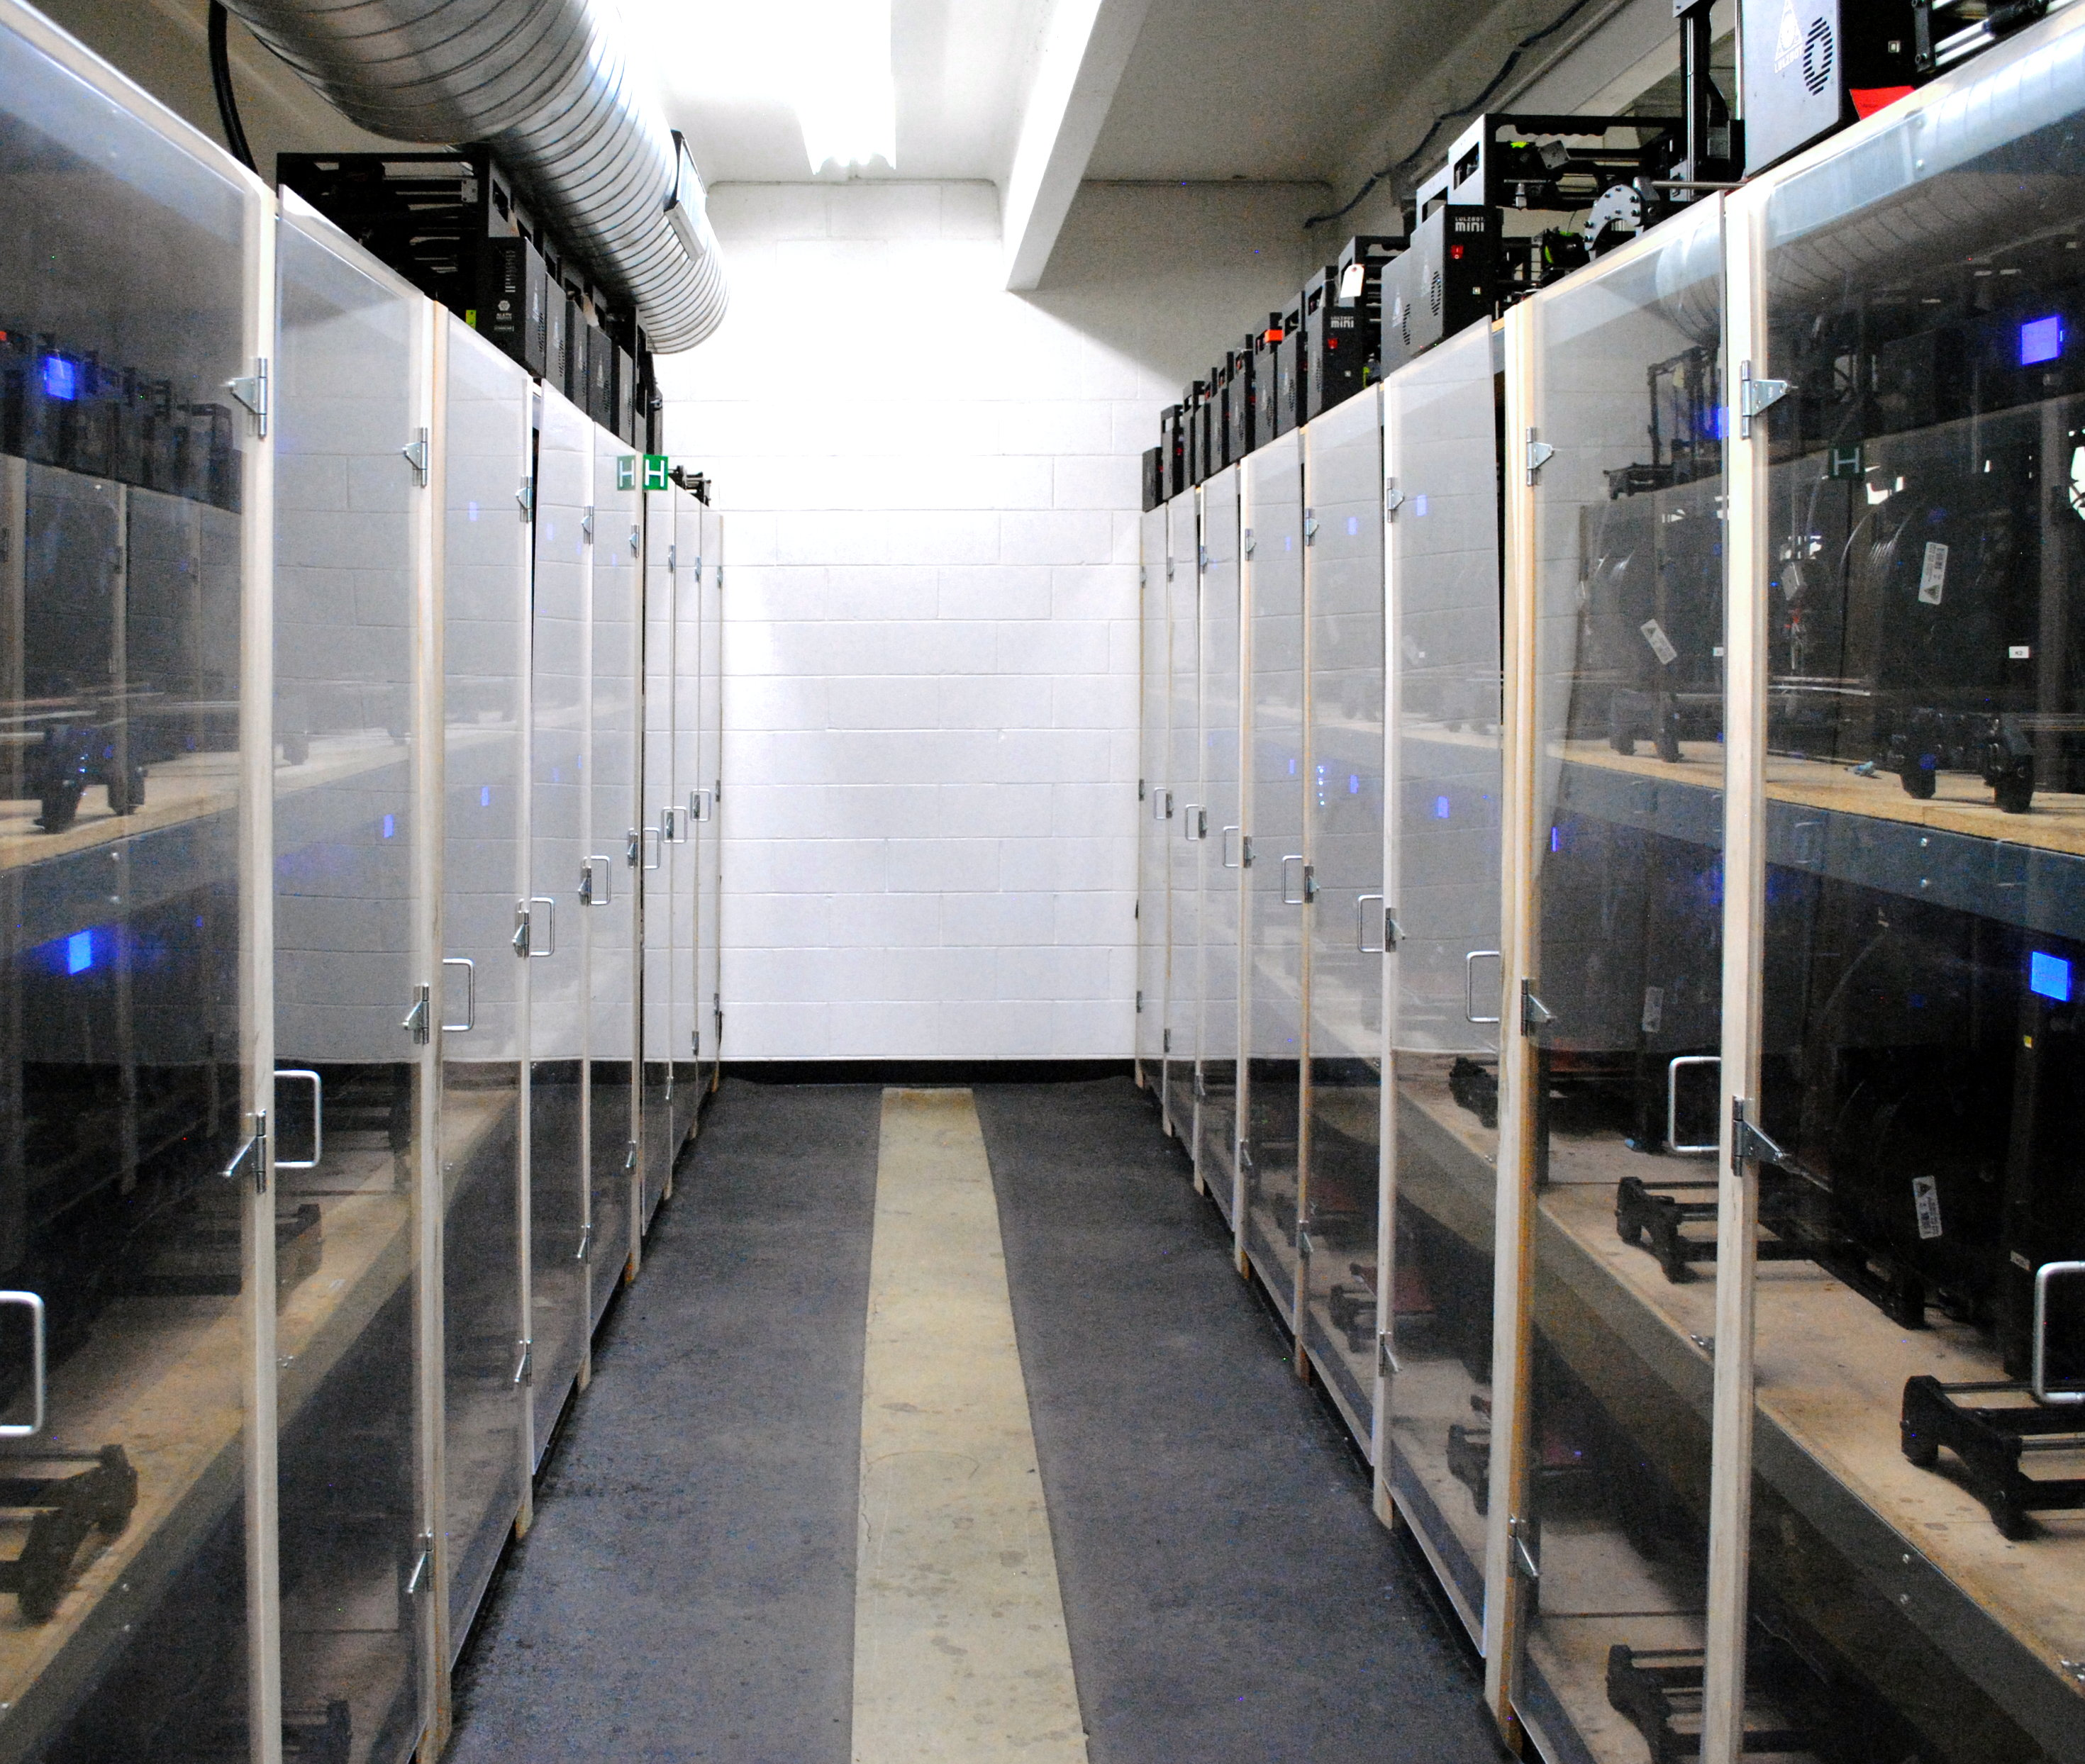
\includegraphics[keepaspectratio=true,height=0.40\textheight,width=1.00\textwidth,angle=0]{cluster/taz-135-node.jpg}
 \caption{Section of 3D Printer Cluster of 135 LulzBot TAZ, April, 2015.}
 \label{fig:taz-135-node}
\end{figure}

